\definecolor{deepblue}{rgb}{0,0,0.5}
\definecolor{deepred}{rgb}{0.6,0,0}
\definecolor{deepgreen}{rgb}{0,0.5,0}
\DeclareFixedFont{\ttb}{T1}{txtt}{bx}{n}{12} % for bold
\DeclareFixedFont{\ttm}{T1}{txtt}{m}{n}{12}  % for normal


\newcommand\realnumberstyle[1]{}


% Python style for highlighting
\newcommand\pythonstyle{\lstset{
		language=Python,
		basicstyle=\ttm,
		otherkeywords={self},             % Add keywords here
		keywordstyle=\ttb\color{deepblue},
		emph={MyClass,__init__},          % Custom highlighting
		emphstyle=\ttb\color{deepred},    % Custom highlighting style
		stringstyle=\color{deepgreen},
		frame=tb,                         % Any extra options here
		showstringspaces=false 
		xleftmargin=\dimexpr\fboxsep-\fboxrule,
		xrightmargin=\dimexpr\fboxsep-\fboxrule,
		gobble=16 ,
		numbers=left
	}}
	
	
	% Python environment
	\lstnewenvironment{python}[1][]
	{
		\pythonstyle
		\lstset{#1}
	}
	{}

\mychapter{1}{Decision Trees}
	\label{ch:dt}
	\section{Esercizio 1}
		\label{sec:es1}
		\subsection{}
		%una tipologia  di apprendimento assistito.utilizzando tale tipo di apprendimento abbiamo che il nostro agente intelligente e' in grado di prendere decisioni basandosi sull'albero di decisioni, costruito  classificando i vari esempi che gli sono stati forniti, cercando di estrarre le informazioni necessarie eliminando quelle superflue e ridondanti
		
		In questo primo lavoro di gruppo, vogliamo soffermarci sugli alberi di decisione usati per il Machine Learning, un tipo di apprendimento assistito, in cui si va a creare un albero che classifica vari esempi e cerca di estrarre le informazioni necessarie, eliminando quelle superflue o ridondanti.
		\newline
		Come primo esempio di classificazione, prendiamo un insieme di dati che riguardano vari tipi di iris, caratterizzabili da quattro attributi: lunghezza del sepalo, larghezza del sepalo, lunghezza del petalo, larghezza del petalo, espresse tutte in cm,  il nostro intero set di dati è formato 150 esempi, decidiamo di usare un 
		40\% per il training, quindi per l' apprendimento, ed un 60 \% per il test.
		%espresse in cm.La dimensione complessiva del dataset che abbiamo utilizzato e' di 150 elementi. Nel primo test del codice che abbiamo effettuato abbiamo deciso di utilizzare il ... tali set di dati sono costruiti automaticamente da una funzione da noi scritta che crea i data set scegliendo elementi random
		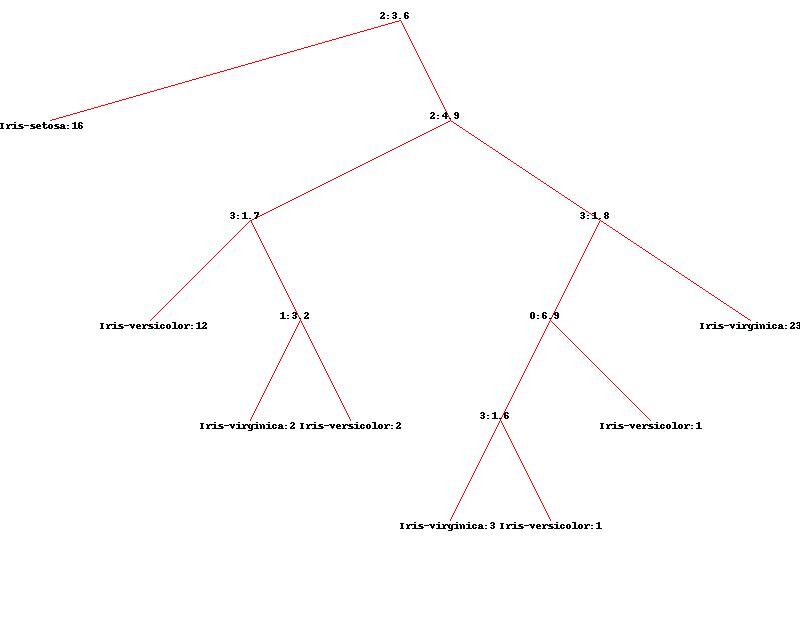
\includegraphics[scale=0.37]{iris.jpg}
		
		 Come si %evince
		  vede dalla figura, il nodo scelto come radice è la terza colonna(colonna numero 2 da programma, perché la numerazione effettuata dal codice della classificazione rimarca quella delle liste in python) ed il valore che  minimizza la funzione d' entropia è 3.6, infatti ci permette di caratterizzare già 16 esempi.L'albero con l' informazioni di training, riesce a classificare tutti gli esempi, anche se il contenuto informativo non è alto, perché come vediamo, un attributo non riesce a caratterizzare nettamente un gruppo di esempi,infatti più volte sono richiamati per splittare nuovamente i dati, aumentando così la profondità dell' albero.Quest' ultimo,per tale ragione non è generico, molto probabilmente %se gli carichiamo un dataset con dati molto diversi da quelli con cui e' stato effettuato il training non ci offrira' ottimi risultati...
		  non ci offrirà ottimi risultati con dati a lui sconosciuti, si potrebbe pensare di applicare una potatura per renderlo più semplice, affinché da poter rispettare il rasoio di Okam.
		\newline
		\newline
		%li separeri come paragrafo uno chiamerei iris e uno fughi 
		Ora invece ci concentriamo su un diverso data set relativo ai funghi, caratterizzato da ben 22 attributi, utilizziamo sempre la stessa percentuali di dati per il training ed il test set.
		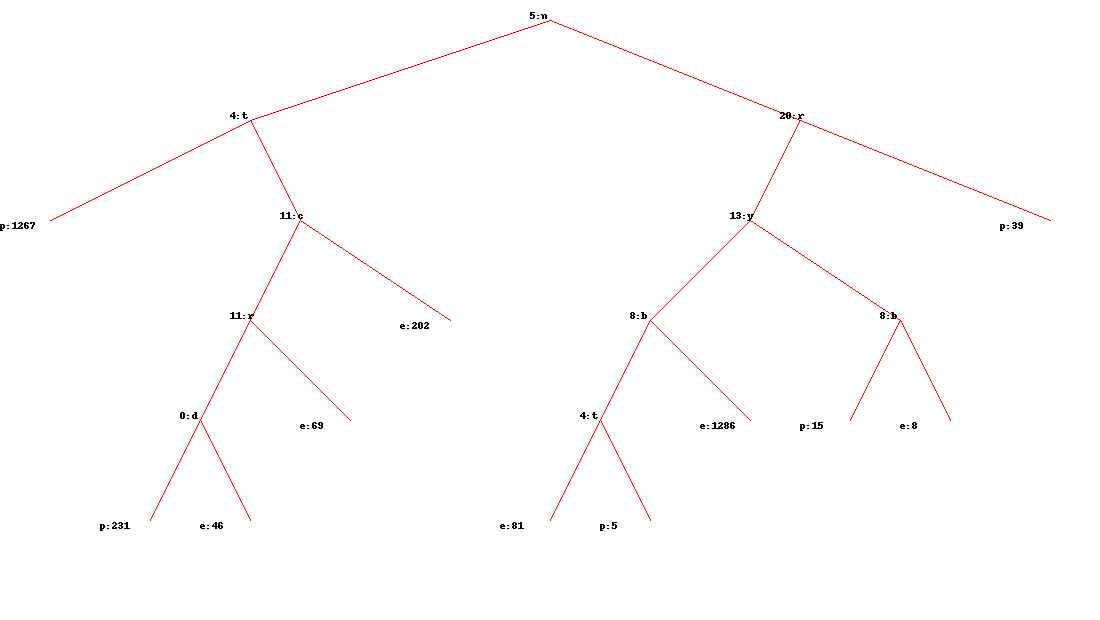
\includegraphics[width=.9\textwidth, height=0.63\textheight]{mushroom.jpg}		
		L' albero,come si può osservare non è in grado di classificare gli esempi distintamente.
		%in seguito a vari test effettuati con diversi elementi che componevano il training set, i risultati sono appartsi sempre inconcludenti in quanto c'era sempre un numero di nodi maggiore di 3 che portano a decisioni ambuigue, nel nodo foglia c'erano piu' risultati.Per tanto visto che stiamo studiando tale materia abbiamo deciso di soffermarci su tali risultati giungendo alle seguenti conclusioni enumerato quello che sta dopo. 
	    Tale risultato può essere conseguenza dal fatto che il numero di esempi usato per il training sia troppo piccolo, quindi non capace di permettere di discriminare appieno una scelta, oppure gli attributi utilizzati non sono abbastanza rappresentativi, non riuscendo a classificare appieno i vari esempi, quindi bisognerebbe introdurre altri attributi oppure modificare quelli usati,in questo stato l' albero può portare a decisioni includenti.
		\subsection{}
		In questo esempio mostreremo al variare del training set e del data set il cambiamento valore della performance dell' albero visualizzando tramite un grafico.
		\newline
		Il data set che andremo ad utilizzare è stato preso da un censimento, per identificare le persone che guadagnano più di cinquanta mila dollari all' anno.
		Le righe di codice adibite alla generazione del grafico sono quelle scritte in questa funzione:
		\begin{python}
		def fperformance(data):
			testc=data
			percent=10
			p=[]
			perc=[]
			t=[]
			numdati=(int)((float)(len(testc))/100*percent);
			for i in range(0,5):
				(train,testc)=createdataset(testc,numdati,t)
				t=t+train;
				tree=buildtree(t)
				p=p+[performance(tree,testc)]
				perc=perc+[percent]
				percent=percent+10;
				line,=plt.plot(perc,p,'r-')
			plt.xlabel('percentuale dati training')
			plt.ylabel('percentuale successi')
			line.set_antialiased(False)
			plt.show()
		\end{python}
	%passiamo ora a descrivere cosa fa questa funzione come prima cosa effettua una copia del dataset che gli e' stato ricevuto dopodiche' inizializza una serie di liste a supporto delle operazioni successive. farei una descrizione per linee di codice, metterei il codice per riga sia sopra che sotto commentando
		la funzione essenzialmente dopo aver fatto una copia dei dati passati, fatto un paio di inizializzazione di liste che ci occorrono per il plot dei dati e aver determinato il numero di elementi da aggiungere al training set(togliendoli al test set), iterativamente per 5 volte divide i dati in train set e test set, dopo di che il train viene assegnata ad una lista t che incrementa ad ogni variazione e scritta su file da createdataset, viene costruito l' albero, se ne calcola il valore di performance, richiamando al suo interno la funzione classify che ritorna la classificazione  fatta dall ' albero con gli attributi dell' esempio e confrontandoli con il valore del test, se l' albero è riuscito a classificare bene l' esempio allora si avrà un riscontro positivo, altrimenti negativo, alla fine performance ritorna la percentuale di positivi sul numero di test effettuati.Dopo di che si aggiungono i punti alla linea per il plot e alla fine viene mostrata su schermo, un esempio di curva è questo:
		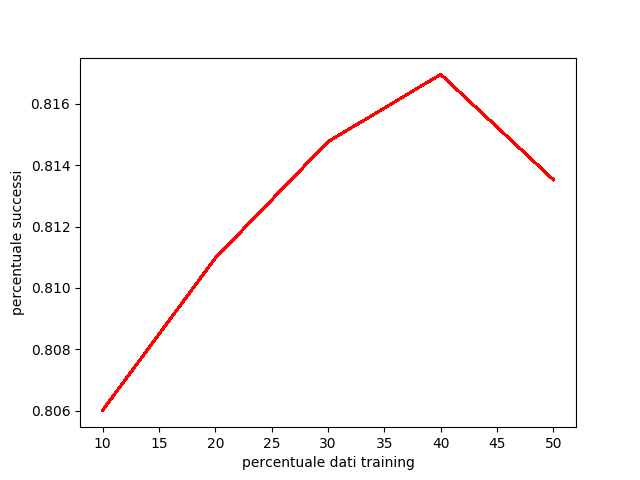
\includegraphics[scale=0.86]{performance.png}
		%evince 
		Come si vede dal grafico la nostra percentuale di apprendimento migliora fino al 40\% dopodichè si percepisce un degrado dell'apprendimento quando arriviamo al 50\% di dati utilizzati per il training-set.
		\newline
		 Su tale risultato siamo giunti alla seguente considerazione "aumentando il training-set si è giunti alla realizzazione di un albero più specifico e di conseguenza meno capacità di classificare gli esempi".
		 Dalla figura che mostra l'andamento della curva di apprendimento, si intuisce che la rappresentazione dell'ambiente così descritto dai data-set è ridondante.
		  Infatti la crescita è lenta, al crescere del training-set dal 10\% al 50\% si evince che l'aumento è di circa del 1\%.
		  Per migliorare la qualità dell'albero di decisione si potrebbero rimuovere alcuni attribbuti, in modo tale da incrementare la ripidità della curva.
		  Il problme è quale di questi attributi bisogna rimuovere?
		  \newline
			Ovviamente  bisognerebbe testare altre configurazioni dell' ambiente in cui abbiamo un numero di attributi minore.
		\subsection{}
		
		%tali tecniche di apprendimento mirano alla formulazione di una funzione h che approssimi la funzione f, dove ricordiamo che f è la funzione condizione azione che si vorrebbe apprendere. la costruione di h avviene 
			Un agente in grado di apprendere mediante alberi di decisione fonda questo suo processo su principi di apprendimento induttivo (\textsf{inductive learning}). L'apprendimento induttivo è una forma di apprendimento basata sull'induzione a partire da esempi dati. Esso, data una collezione di esempi (\textsf{training set}) della funzione \textsf{target} \emph{f} che si vorrebbe imparare, mira a restituire una funzione \emph{h} (\textsf{hypothesis}) che approssimi la \emph{f}, anche se non è detto che riesca a trovare una che l' approssimi bene nello spazio delle funzioni. Concettualmente, il criterio nella determinazione di \emph{h} tra le differenti funzioni dello spazio delle ipotesi dovrebbe essere legato, più che alla consistenza nello spiegare i dati, alla bontà dell'approssimazione e quindi alla capacità di generalizzazione per predire esempi non ancora incontrati. In questo senso, l'agente agisce in modo razionale poichè cerca di \textbf{decidere come comportarsi in situazioni a lui sconosciute basandosi su quelle già note}. Possiamo individuare proprio in questo aspetto una \textbf{forma di intelligenza}, determinata dall'agire razionalmente.
		\subsection{}
			Le procedure di \textsf{Decision Tree Learning} consentono la costruzione di un albero di decisione "piccolo", consistente con gli esempi forniti in input per la costruzione di tale struttura. Ogni nodo interno all'albero corrisponde ad una condizione sul valore di un attributo(quindi una decisione), gli archi verso i nodi figli ai possibili valori per quell'attributo(una scelta intrapresa), le foglie alla classificazione(target raggiunto). Si ottiene così, attraverso i \textsf{path} dell'albero, una rappresentazione compatta delle regole di condizione-azione. L'albero di decisione prende in input una situazione descritta da un insieme di attributi e restituisce una decisione, ovvero il valore predetto di uscita per tale input, sulla base del cammino percorso. In questo senso possiamo parlare di apprendimento, poiché, \textbf{alla luce di un dato insieme di esempi, si viene a costituire un albero di decisione dalla ben determinata topologia e legge condizione-azione, utilizzabile per la classificazione di esempi futuri}.
	\section{Esercizio 2}
		\label{sec:es2}
		Il problema descritto è del tipo \emph{non deterministico} e \emph{parzialmente osservabile}, quindi classificabile come \textsf{Contingency Problem}. L'algoritmo di navigazione proposto fa uso di un albero di ricerca con strategia di ricerca in profondità (\textsf{depth-first search}), la quale prevede di espandere primariamente il nodo più profondo non espanso.
		\newline
		 L'alterazione non deterministica delle distanze ci ha spinto a sottolineare l'importanza di \textbf{minimizzare il numero di città percorse} lungo il tragitto verso l'obiettivo. Un maggior numero di città attraversate aumenterebbe probabilisticamente la distanza percorsa. Sarebbe, quindi, auspicabile evitare, o minimizzare, il numero di processi di risalita dell'albero, che prevederebbero il ritorno alle stesse città più volte, e continuare nella navigazione in profondità, sfruttando, nel migliore dei casi, la possibilità di arrivare al \textsf{goal} senza attuare un \textsf{backtracking}. Inoltre, per evitare l'insorgere di cicli, si è previsto di tenere traccia dell'insieme dei nodi già esplorati,mediante l'utilizzo di una lista, ottenendo in definitiva un algoritmo del tipo \textsf{Graph Search}.
La scelta dell'utilizzo della struttura dati lista semplice, è stata dettata dalla natura del problema, in quanto a differenza del problema analogo, ma diverso trattato in classe, in questo esempio le distanze tra le città non sono costanti e quindi la struttura dati lista ordinata in base alla distanza non si adatta a tale tipologia di problema.
